% Chapter 1

\chapter{Deep Learning and Tomographic Image Reconstruction} % Main chapter title

\label{Chapter2} % For referencing the chapter elsewhere, use \ref{Chapter1} 

%----------------------------------------------------------------------------------------
The impact of deep learning has been immense over the last few years in the field of medical imaging (\cite{litjens2017survey, greenspan2016guest}). Medical image reconstruction has also benefited hugely from the various advances in neural network architectures \cite{wang2020deep,yedder2021deep,reader2020deep}. In the specific case of \ac{CT} image reconstruction, there has been active interest in sparse-view and low-dose reconstruction scenarios. While with \ac{PET} reconstruction on the other hand, low-dose imaging and total body imaging have been on the forefront. In both cases, obtaining high quality reconstructed images is a challenging task. Many established model-based iterative methods account for the low-dose and sparse-view settings to remove artifacts and noise from the reconstruction (\cite{nuyts1998iterative,Elbakri2002,liu2013total}). However, these methods require the knowledge of noise and artifacts statistics and generally have longer reconstruction times \cite{kim2014combining}. Deep learning-based methods on the other hand are claimed to achieve reconstructed images with quality on par with iterative techniques and in a much shorter time frame \cite{leuschner2021quantitative}. In this work, the focus has been on \ac{CT} and \ac{PET} image reconstruction. 
Image reconstruction corresponds to the task of mapping raw projection data retrieved from the detector to image domain data. As depicted in Fig~\ref{fig:dl}, one can broadly identify three different categories of approaches for the implementation of deep learning within the framework of medical image reconstruction:
\begin{itemize}
	\item[(i)] methods that use deep learning as an image processing step that improves the quality of the raw data and/or the reconstructed image (\cite{gong2018pet, maier2018deep}); 
	\item[(ii)] methods that embed deep-learning image processing techniques in the iterative reconstruction framework to accelerate convergence or to improve image quality (\cite{xie2019generative,kim2018penalized,gong2019iterative});
	\item[(iii)] direct reconstruction with deep learning alone without any use of traditional reconstruction methods  (\cite{whiteley2019direct,zhu2018image,haeggstroem2018deeprec}).
\end{itemize}

\begin{figure}[!htbp]
	\centering
	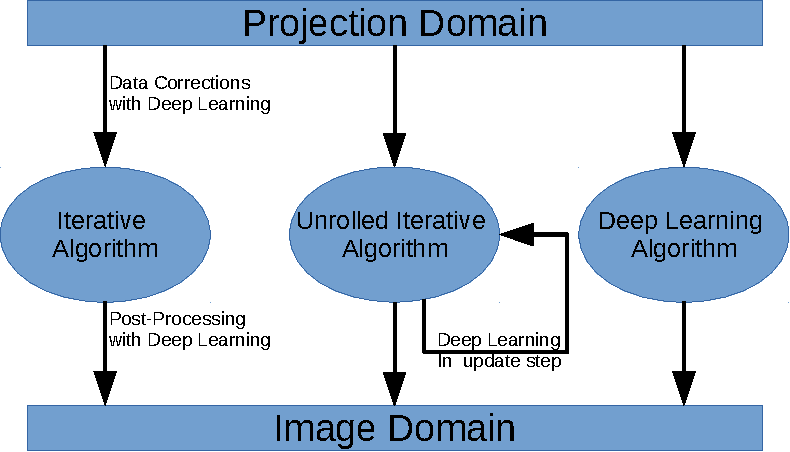
\includegraphics[width=0.8\linewidth]{./Figures/dl_mi.pdf}
	\caption{Deep Learning in Medical Image Reconstruction}
	\label{fig:dl}
\end{figure}


Each of these categories are discussed along with reference to existing state of the art methods for \ac{CT} and \ac{PET} image reconstruction in this chapter. 

\section{Data Corrections or Post-processing}

The use of deep learning for the development of either data corrections or post-reconstruction  image based approaches has shown potential to improve the quality of reconstructed images. While it is possible to train a \ac{CNN} to regress directly from the measurement (raw data) domain to the image domain, the use of \ac{CNN} entirely in one particular domain makes it fast and relatively easy to implement. The motivation behind using deep learning architectures for these processing task is the extremely well documented performance in denoising and super resolution tasks. Data corrections involve improving the measurement data either though denoising or finding missing projection angle data. Post-processing in the image domain on the other hand consists of improving images reconstructed with standard reconstruction methods. 
Corrections in measured data $\boldy$ can be expressed as finding an estimate $\boldyhat$ through a neural network $F$ with parameters $\bm{\theta}$. 
\begin{equation}\label{eq:data_cor}
	\boldyhat = \bm{F}_{\bm{\theta}} (\boldy)
\end{equation} 
The new set of corrected data $\boldyhat$ are then used to reconstruct images through traditional methods. An example of data corrections in \ac{PET} image reconstruction through sinogram repair is proposed by \cite{whiteley2019cnn}, where a \ac{CNN} is utilized to predict missing projection data for total body \ac{PET} image reconstruction. The repaired sinograms eventually improve image reconstruction by standard methods.

In \ac{CT} imaging, missing projection data in sparse-view setting is estimated through neural networks. An example in this regard is proposed in \cite{lee2018deep}, where the authors use U-Net to map sparse-view sinograms to full-view sinograms and then reconstruct the images using \ac{FBP}. Another idea to improve the raw data through scatter correction is proposed in \cite{maier2018deep}. In this work a modified U-Net is used to estimate scatter and correct the raw data in order to improve \ac{CT} images. 

Improvements in the images reconstructed by traditional methods are usually brought about through neural networks designed for denoising or super resolution. An image $\boldxhat$ ($\boldlambdahat$ or $\boldmuhat$) estimated by conventional methods like \ac{FBP} or \ac{OSEM} is improved through a neural network:

\begin{equation}\label{eq:post_pro}
\boldx_{\mathrm{den}} = \bm{F}_{\bm{\theta}} (\boldxhat)
\end{equation} 
where $\boldx_{\mathrm{den}}$ is the post-processed image. Over the years the trend in \ac{PET} imaging has been towards reducing the dose of the radiotracer injected into the patient, which in turn leads to noisier reconstructed images. The approach has been to create datasets with conventional algorithms (like \ac{OSEM}) for both low-dose and normal dose settings and then train a neural network to achieve normal dose quality starting from low-dose images. Apart from the low dose noise problem, in \ac{CT}, improvements in sparse-view imaging through has been an active area of research. The focus here is to reduce the artifacts produced by \ac{FBP} with sparse-view sinograms. These artifacts are either removed by first finding the missing projections and repairing the sinograms or by post-processing the images. In both these scenarios \ac{FBP} is utilized; in the former case neural network corrects the sinograms thereby providing full-view sinograms for reconstruction and in the latter case \ac{FBP} estimated artifact effected images are improved by the neural network.  

Some of the recent developments in post-processing and data corrections for \ac{PET} and \ac{CT} are summarized in Table~\ref{table:pp_PET} and Table~\ref{table:pp_CT}. A short description of the method along with the citation is given in the second column of both the tables. These approaches typically modify an existing neural network architecture to suit the problem they are addressing. U-Net is one of the most utilized architectures as seen in the third column where the base neural network is given. The datasets utilized by each of these is works is mentioned in the final column. Along with proposed modifications of established neural networks, these approaches typically use loss functions consisting of multiple components. The authors in \cite{gong2018pet} used perceptual loss along with \ac{MSE} to preserve qualitative and quantitative accuracy of the reconstructed images. The work proposed by \cite{whiteley2020fastpet} uses \ac{MSSIM} along with perceptual loss and \ac{MAE}. Another strategy used is pre-training on simulated data followed by fine-tuning on real patient data. Data corrections in the form of scatter correction of the sinogram data is proposed in \cite{qian2017deep}. The authors use \ac{CNN} followed by \ac{FC} layers in their approach. In \ac{CT} imaging there are works that do denoising of low-dose sinograms (\cite{ma2021sinogram,zhu2020low}) and also finding the missing projections in sparse-view sinograms (\cite{lee2018deep}). The same problem is tackled in the image domain through denoising (\cite{yang2018low}) and artifact removal for sparse-view problem (\cite{jin2017deep,xie2018artifact,zhang2018sparse}).
\begin{table}[ht!]
	\centering
	\caption{Summary of recent works on data corrections and post-processing approaches in \ac{PET}}
	\label{table:pp_PET}
	\scriptsize
	\begin{tabular}{||c|c|c|c||} 
		\hline
		Sl.No.    & Method             & Base Neural  & Dataset        \\ %[0.5ex] 
		          &                    &  Network     &                \\
		\hline\hline
		1         & \cite{gong2018pet} & \ac{CNN} with residual & BrainWeb and XCAT  \\     
		          &  Low-dose Image    &  blocks                & phantoms; Fine-tuning/testing  \\ 
		          &   Denoising        & & with real patient data       \\ 
		\hline
		2         &  \cite{whiteley2020fastpet}& U-Net with residual & Real PET/CT data \\
		          & Histo Image        & blocks      &        \\
		          & Correction         &                &        \\
		\hline  
		3         & \cite{zhao2020study}& Cycle GAN    & Real PET/CT data  \\ 
       	          & Low-dose Image      &              &                   \\ 
       	          & Denoising           &              &                   \\ 
       	\hline
       	4         & \cite{qian2017deep} & CNN with fully    & Monte Carlo simulations  \\ 
                  & Sinogram Scatter    & connected layer   & with phantoms            \\ 
       	          & Correction          &                   &                          \\ 
       	\hline
       	5         & \cite{hong2018enhancing}& Deep residual CNN & Digital phantoms  \\ 
       	          & Single Image Super      &                   &             \\ 
       	          & Resolution for sinograms&                   &                          \\ 
       	\hline
       	6         & \cite{sanaat2021deeptofsino}&   ResNet       & Real TOF-PET/CT data  \\ 
       	          & Low-dose to full-dose    &                   &             \\ 
       	          & sinogram synthesis    &                      &                          \\ 
       	\hline
       	
	\end{tabular}
	
\end{table}

\begin{table}[ht!]
	\centering
	\caption{Summary of recent works on data corrections and post-processing approaches in \ac{CT}}
	\label{table:pp_CT}
	%\footnotesize
	\scriptsize
	\begin{tabular}{||c|c|c|c||} 
		\hline
		Sl.No.    &       Method             & Base Neural          & Dataset        \\ %[0.5ex] 
            	  &                          &    Network                      &                \\
		\hline\hline
		1         & \cite{lee2018deep}       &   Residual U-Net     & Simulated projections          \\     
		          &  Sinogram synthesis      &                      & from real patient data         \\ 
		          &   for sparse-view CT     &                      &                                \\ 
		\hline
		2         &  \cite{jin2017deep}      & Residual U-Net       & Phantom and Real patient       \\
		          & Artifact removal in      &                      &   data along with projections  \\
		          & sparse-view reconstructed images&               &                                \\
		\hline  
		3         & \cite{xie2018artifact}   & Improved GoogleNet   & Simulated projections          \\ 
		          & Artifact removal in      &                      & from real data                 \\ 
		          & sparse-view reconstructed images&               &                                \\ 
		\hline
		4         & \cite{zhang2018sparse}    & DeneNet with        & Simulated projections          \\ 
		          & Artifact removal in       & deconvolutions      & from real data                 \\ 
		          & sparse-view reconstructed images&               &                                \\ 
		\hline
		5         & \cite{ma2021sinogram}     & Attention residual  & Real data along with           \\ 
		          & Low dose sinogram         &  dense CNN          & projections                    \\ 
		          & denoising                 &                     &                                \\ 
		\hline
		6         & \cite{yang2018low}        &    Wasserstein-GAN & Real data along with            \\ 
		          & Low-dose image            &                    & projections                     \\ 
		          & denosing                  &                    &                                 \\ 
		\hline
		7         & \cite{zhu2020low}         &  Three-segment network  & Real data along with            \\ 
		          & Simultaneous sinogram and &  ADAPTIVE-NET      & projections                     \\ 
	 	          & image domain denoising    &                    &                                 \\ 
		\hline
		
	\end{tabular}
	
\end{table}

An important aspect of the methods discussed in this section is that they all claim to provide fast reconstructed images using well established neural network architectures. This also stems from the fact that most of these approaches start with an image estimate that is also obtained with a relatively faster conventional method, like \ac{FBP} for \ac{CT} and \ac{OSEM} for \ac{PET}. These fast estimates are usually very noisy or artifact ridden. These approaches rely on the neural network to handle the noise and artifacts. The attractiveness of these methods is the simplicity, ease of implementation and the lack of requirement of large datasets of raw detector data. 

\section{Hybrid Methods}

The methods mentioned in this section and the next, are directly involved in the reconstruction process, rather than being exclusive to data corrections or post-reconstruction processing. The hybrid methodology for image reconstruction combines model-based and neural network approaches exploring the benefits of both methods. Data-driven information learned by a neural networks can be incorporated into an iterative algorithm through the regularization term. \cite{gong2019iterative} used a modified version of the U-Net comprising of multi-channel input to represent \ac{PET} images.
\begin{equation}\label{eq:iter_CNN}
\boldlambda = \bm{F}_{\bm{\theta_{\mathrm{fixed}}}}(\bm{z})
\end{equation} 
where $\bm{F}_{\bm{\theta_{\mathrm{fixed}}}}$ represents the trained denoising neural network (modified U-Net) with fixed trainable parameters $\theta_{\mathrm{fixed}}$. The \ac{PET} reconstruction model (from \ref{eq:PET}) can be modified to incorporate \ref{eq:iter_CNN}. 

\begin{equation}\label{eq:mod_PET}
	\boldybar(\boldlambda) = \boldA \bm{F}_{\bm{\theta_{\mathrm{fixed}}}}(\bm{z}) + \bm{r}
\end{equation}
The unknown image $\boldlambda$ can be estimated using the maximum likelihood criterion:
\begin{equation}\label{eq:iter_CNN2}
\boldlambdahat = \bm{F}_{\bm{\theta_{\mathrm{fixed}}}}(\bm{\hat{z}})
\end{equation} 
\begin{equation}
\boldlambdahat=\underset{\boldlambda \ge 0}{\operatorname{argmin}} \; L(\bm{z})
\end{equation}

In order to ease the difficulty of solving the above due to the non-linearity of the neural network, the authors adapted a constrained version of the above:

\begin{equation}\label{constr}
 	\operatorname{max} \; L(\bm{\boldlambda});  \; \mathrm{s.t.} \; \boldlambda = \bm{F}_{\bm{\theta_{\mathrm{fixed}}}}(\bm{\hat{z}})
\end{equation}
To solve the above optimization problem the authors used the augmented Lagrangian format:
\begin{equation}
L_{\rho}=L(\boldlambda)-\frac{\rho}{2}\|\boldlambda-\bm{F}_{\bm{\theta_{\mathrm{fixed}}}}(\bm{z})+\bm{\gamma}\|^{2}+\frac{\rho}{2}\|\bm{\gamma}\|^{2},
\end{equation}
The authors used the \ac{ADMM} algorithm to split the above into three steps:

\begin{equation}
\boldlambda^{n+1}=\underset{\boldlambda}{\arg \max} \; L(\boldlambda)-\frac{\rho}{2}\left\|\boldlambda-\bm{F}_{\bm{\theta_{\mathrm{fixed}}}}(\bm{z})^{n}+\bm{\gamma}^{n}\right\|^{2}
\end{equation}

\begin{equation}
\bm{z}^{n+1}=\arg \min \left\|\bm{F}_{\bm{\theta_{\mathrm{fixed}}}}(\bm{z})-\left(\boldlambda^{n+1}+\bm{\gamma}^{n}\right)\right\|^{2}
\end{equation}

\begin{equation}
\bm{\gamma}^{n+1}=\bm{\gamma}^{n}+\boldlambda^{n+1}-\bm{F}_{\bm{\theta_{\mathrm{fixed}}}}(\bm{z})^{n+1}
\end{equation}


The paper by Gong et al. used a modified U-Net to represent images within the iterative reconstruction framework for \ac{PET} images. The deep learning architecture was trained on low-dose reconstructed images as input and high-dose reconstructed images as the output. The work by Xie et al. further extended this work by replacing the U-Net with a \ac{GAN} for image representation within the iterative framework. Kim et al incorporated a trained denoising convolutional neural network (DnCNN) along with a novel local linear fitting function into the iterative algorithm. The DnCNN which is trained on data with multiple noise levels improves the image estimate at each iteration. They used simulated and real patient data in their study. In \cite{gupta2018cnn}, a U-Net is used to encode the prior, i.e., to project the current estimate to the prior image set while gradient descent enforces measurement consistency. Neural networks can be also used to replace traditional operators in optimization strategies as shown by \cite{adler2018learned}. The reconstruction using these hybrid methods can be computationally expensive since it requires running an optimization procedure at test time.

\section{Direct Reconstruction with Deep Learning}

An alternative approach is using deep learning-based methods to directly map from projection to image space. Essentially neural network can be modeled to approximately learn  the inverse mapping from measurement($y$) to image ($x$). As represented in Fig~\ref{fig:direct}, a neural network ($F$) with parameters ($\theta$) can be represented as:

\begin{equation}\label{eq:direct}
x=\boldsymbol{F}_{\widehat{\boldsymbol{\theta}}} \boldsymbol{y}
\end{equation}

The challenge in this approach is the management of data and the number of parameters required for learning the mapping. Due to these challenges, this approach has been less explored compared to the two approaches discussed above. 


\begin{figure}[!htbp]
	\centering
	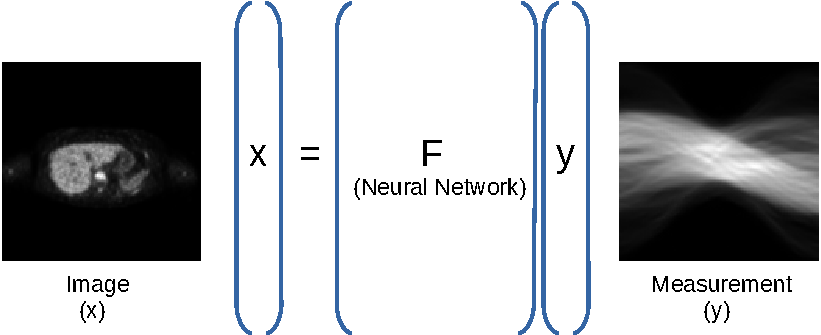
\includegraphics[width=0.8\linewidth]{./Figures/direct-crop.pdf}
	\caption{Direct image reconstruction with deep learning}
	\label{fig:direct}
\end{figure}

The deep learning architecture proposed by Zhu et al.~\cite{zhu2018image} called AUTOMAP uses \ac{FC} layers (which encode the raw data information) followed with convolutional layers.
The first three layers in this architecture are \ac{FC} layers with dimensions $2n^2$,$n^2$ and $n^2$ respectively where $n\times{}n$ is the dimension of the input image. The AUTOMAP requires the estimation of a huge number of parameters which makes it computationally intensive. Although initially developed for \ac{MRI}, AUTOMAP has been claimed to work on other imaging modalities too. Brain images encoded into sensor-domain sampling strategies with varying levels of additive white Gaussian noise were reconstructed with AUTOMAP.  Within the same concept of using \ac{FC} layers' architectures a three stage image reconstruction pipeline called DirectPET has been proposed to reduce associated computational issues  \cite{whiteley2019direct}. The first stage down-samples the sinogram data, following which a unique Radon transform layer encodes the transformation from sinogram to image space. Finally the estimated image is improved using a super resolution block. This work was applied to full body \ac{PET} images and remains the only approach that can reconstruct multiple slices simultaneously (up to 16 images). DeepPET is another approach implemented on simulated images using encoder-decoder architecture based on the neural network proposed by the visual geometric group \cite{haeggstroem2018deeprec}. Using realistic simulated data, they demonstrated a network that could reconstruct images faster, and with an image quality (in terms of root mean squared error) comparable to that of conventional iterative reconstruction techniques.  


In \cite{li2019learning} the authors proposed an architecture termed iCT-Net  consisting of $12$ layers that are a combination of convolutions and modified fully-connected layers. The $12$ layers are separated into segments and are trained separately before being combined for end-to-end training. To reduce the number of parameters in learning the mapping for full resolution \ac{CT} reconstruction, \cite{fu2019hierarchical} proposed a breakdown of the problem into smaller fragments that can be mapped onto a hierarchical network architecture. The approach proposed in \cite{ye2018deep} converts the sinogram data into a stack of back projections for each angle, which are then fed into a \ac{CNN}. The spatial in-variance of the \ac{CNN} is exploited to learn the mapping from these single view stacked back projections onto reconstructed images. Currently, we observe that adversarial networks are increasingly used in scenarios with high-resolution images. In \cite{thaler2018sparse} a Wasserstein generative adversarial network \cite{arjovsky2017wasserstein} is proposed for sparse-view \ac{CT} image reconstruction. The authors used a combination of $L_1$ loss and adversarial loss to train their network. The generator in their work is a U-Net and the discriminator a typical classification \ac{CNN}. It is to be noted that the authors performed their experiments on down-sampled images of resolution $128\times 128$. Another methodology referred to as DUG-RECON \cite{kandarpa2020dug}, used a three-stage network to divide the image reconstruction problem into denoising, domain mapping and resolution improvement. They used a residual UNet for denoising the sinograms, then a double-UNet architecture to map the sinogram to image, and finally a super ResNet to improve image estimate. The approach was tested with both \ac{PET} and \ac{CT} data. 




